%%%%%%%%%%%%%%%%%%%%%%%%%%%%%%%%%%%%%%%%%%%%%%%%%%%%%%%%%%%%%%%%%%%%%%%%%%%%%%%%%%%%%%%%%
%%                                                                                     %%
%%                This file is part of the CAPH Compiler distribution                  %%
%%                            http:%/caph.univ-bpclermont.fr                           %%
%%                                                                                     %%
%%                                  Jocelyn SEROT                                      %%
%%                         Jocelyn.Serot@univ-bpclermont.fr                            %%
%%                                                                                     %%
%%         Copyright 2011-2018 Jocelyn SEROT.  All rights reserved.                    %%
%%  This file is distributed under the terms of the GNU Library General Public License %%
%%      with the special exception on linking described in file ..%LICENSE.            %%
%%                                                                                     %%
%%%%%%%%%%%%%%%%%%%%%%%%%%%%%%%%%%%%%%%%%%%%%%%%%%%%%%%%%%%%%%%%%%%%%%%%%%%%%%%%%%%%%%%%%

\chapter{Image processing}
\label{cha:cl-ip}

This chapter describes the implementation, simulation and synthesis, using the command-line
interface, of the \emph{Sobel} application introduced in Chapter~\ref{cha:lang-ip}. 

The code of this application has been given in Listing.~\ref{lst:sobel-full}. The related project
can be found in the directory \verb|examples/primer/sobel| of the distribution.

\section{Simulation using the interpreter}
\label{sec:simulation-3}

The simulation process is completely similar to the one described in Chapter~\ref{cha:cl-images}.
The project description file is reproduced in Listing~\ref{lst:sobel-proj}.

\begin{lstlisting}[style=MakeStyle,caption={Project file for the program of in Listing.~\ref{lst:sobel-full}},label={lst:sobel-proj}]
DOT_OPTS = -D ifile=pcb.pgm -D threshold=80 -suppress_cast_warnings
SIM_OPTS = -D ifile=pcb.pgm -D threshold=80 -suppress_cast_warnings -abbrev_dc_ctors -warn_channels -dump_channel_stats
SC_OPTS = -D ifile=pcb.pgm -D threshold=80 -suppress_cast_warnings -sc_abbrev_dc_ctors -sc_stop_when_idle 1000 -sc_dump_fifo_stats
VHDL_OPTS = -D ifile=pcb.pgm -D threshold=80 -suppress_cast_warnings -vhdl_annot_file sobel_fifo_stats.dat
GHDL_RUN_OPTS = --stop-time=160000ns
\end{lstlisting}
%$

The \verb|-D| option is used is give values to the symbols named \verb|%ifile| and \verb|%threshold|
in the source code. 

The option \verb|-suppress_cast_warnings| is used to omit warning messages
which are emitted when compiling the \verb|fabs| function and which, in this context, can be safely
ignored.

The \verb|-warn_channels| option is set in order to detect channel overflows and the
\verb|-dump_channel_stats| is set in order to check channel usage after run. 

\medskip The \verb|.procs| file for this application, given in Listing~\ref{lst:sobel-procs}, is
similar to that given in the previous chapter. It simply tells how to convert from and to PGM format
for the input and output images.

\begin{lstlisting}[style=MakeStyle,caption={File
    \texttt{sobel.procs} for the \texttt{sobel} program of
    Listing~\ref{lst:sobel-full}},label={lst:sobel-procs}]
PRE_PROC = pgm2txt -abbrev pcb.pgm pcb.txt
POST_PROC = txt2pgm -abbrev 255 sim/result.txt sim/result.pgm
\end{lstlisting}

\medskip
Simulation is performed, as usual with the following sequence of commands :

\begin{lstlisting}[style=BashInputStyle]
# caphmake
# make sim.makefile
# make sim.run
\end{lstlisting}

It produces the following result\footnote{Warning, this can take a few seconds} :

\begin{lstlisting}[style=BashOutputStyle]
make -f Makefile.sim run CAPH=/usr/local/caph
/usr/local/caph/bin/pgm2txt -abbrev pcb.pgm pcb.txt
/usr/local/caph/bin/caphc -sim -I /usr/local/caph/lib/caph -I /usr/local/caph/lib/caph -D ifile=pcb.pgm -D threshold=80 -suppress_cast_warnings -abbrev_dc_ctors -warn_channels -dump_channel_stats main.cph
...
Wrote file ./result.txt
W3: occ=0/256 max=2
W2: occ=140/256 max=140
W1: occ=140/256 max=140
W6: occ=0/256 max=2
W5: occ=140/256 max=140
W4: occ=140/256 max=140
W8: occ=0/256 max=2
W7: occ=0/256 max=2
W9: occ=0/256 max=2
W10: occ=0/256 max=2
\end{lstlisting}

Displaying the output image (Fig.~\ref{fig:sobel-result}-b) is obtained by invoking

\begin{lstlisting}[style=BashInputStyle]
# make sim.show
\end{lstlisting}

\medskip
The maximum occupation reported for channels \verb|W1|, \verb|W2|, \verb|W5| and \verb|W4| is worth
to be noted. The corresponding channels are used by the \verb|conv233| actor to memorize the two
previous lines when computing the convolution\footnote{These channels are those ``looping around''
  the \texttt{conv233} actors in Fig.~\ref{fig:sobel-full}.}. The maximum occupation value
corresponds here to the width in pixels of the input image (140). No overflow occured because the
default depth of channels in simulation is 256. Should we have used a larger image (ex: $512 \times
512$), it would have been necessary to adjust this depth with the \verb|-chan_cap| option.

\begin{figure}[htbp]
  \centering
  \begin{tabular}[c]{cc}
 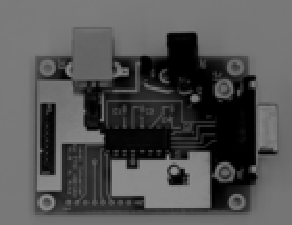
\includegraphics[width=0.3\textwidth]{./figs/pcb.pdf} &
 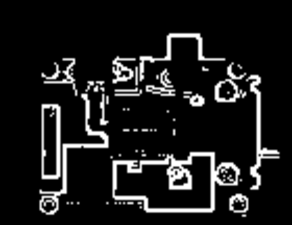
\includegraphics[width=0.3\textwidth]{./figs/pcb-res.pdf} \\
 a & b
  \end{tabular}
  \caption{Input and output images after simulation for the program given in Listing.~\ref{lst:sobel-full}}
  \label{fig:sobel-result}
\end{figure}

\section{Simulation using the SystemC backend}

SystemC simulation is performed exactly as detailed is Sec~\ref{sec:simul-using-sysc-2} (\verb|make systemc.makefile; make systemc.run|) with some
specific options, as shown in Listing~\ref{lst:sobel-proj}. The \verb|-sc_stop_when_idle| option is used to automatically
stop the simulation after a given period of inactivity (1000 ns here, \emph{i.e.} 100 clock
cycles\footnote{The default clock period is 10 ns when using the SystemC backend. This can be
  adjusted with the \texttt{sc\_clock\_period} option.}). The \verb|-sc_dump_fifo_stats| option is
used to get a precise report on FIFO occupation in order to tune the VHDL backend. The resulting
file, \verb|sobel_fifo_stats.dat| is reproduced in Listing~\ref{lst:sobel-sysc-fifos}. 
A visual inspection of the result image shows that it identical to the one obtained using the
interpreter. 

\begin{lstlisting}[style=MakeStyle,caption={Application-specific \texttt{Makefile} for simulating
    wth SystemC the application given in Listing.~\ref{lst:sobel-full}},label={lst:sobel-makef-sysc}]
SC_OPTS = -I $(CAPHLIB) -sc_abbrev_dc_ctors -sc_stop_when_idle 1000 -suppress_cast_warnings -sc_dump_fifo_stats -D ifile=pcb.txt -D threshold=80 
\end{lstlisting}
%$

\begin{lstlisting}[style=CaphStyle,caption={File \texttt{sobel\_fifo\_stats.dat} produced by the SystemC backend for 
    the application given in Listing.~\ref{lst:sobel-full}},label={lst:sobel-sysc-fifos}]
w11 fifo_size = 3
w3 fifo_size = 3
w2 fifo_size = 142
w1 fifo_size = 142
w6 fifo_size = 3
w5 fifo_size = 142
w4 fifo_size = 142
w8 fifo_size = 3
w7 fifo_size = 3
w9 fifo_size = 3
w10 fifo_size = 3
\end{lstlisting}
%$

\section{Simulation using the VHDL backend}

Again, this is very similar to what has been described in the previous chapter. The relevant line in
the project file concerns the \verb|VHDL_OPTS| macro. The \verb|-vhdl_annot_file| option is crucial
here. It gives the name of the annotation file generated by the
previous SystemC execution (\verb|sobel_fifo_stats.dat| here) to ensure correct sizing of the
FIFOs in the final VHDL design (by default, FIFOs have a depth of only 4). Concerning the
\verb|GHDL_RUN_OPTS| macro,  the value specified for
the \verb|--stop-time| option has here been derived from the final time reported by the execution of
the SystemC code (154340 ns). Simulation is a bit longer than with SystemC (about ten seconds) and
produce the same result image.

\section{VHDL synthesis}
\label{sec:vhdl-synthesis-4}

Synthesis results for the application described by the \verb|main_net.vhd| toplevel file on a Cyclone III
FPGA with Quartus II are as follows :
\begin{itemize}
\item total logic elements : 828/119088 ($<1\%$) (combinational function : 682, dedicated logic registers : 512)
\item total memory bits : 6864/3981312 ($<1\%$)
\item IO pins : 23
\item maximum clock frequency : 63.7 MHz
\end{itemize}

\section{Centered \emph{vs.} shifted convolution}
\label{sec:slight-variation}

As evidenced by Eq.~(\ref{eq:conv233}), the \verb|conv233| actor used in the previous sections
implements a so-called \emph{shifted} convolution : the output image is actually ``shifted'' one
line down and one pixel right relatively to the input image. This can be easily explained by the
fact that, since this actor operates on-the-fly on the input data streams, it can only use pixels
which are ``behind'' the current pixel. This is illustrared in Fig.~\ref{fig:shifted-conv}-a, in
which the current pixel is $y_{ij}$ and the ``past'' pixels are those shaded in gray. In this
context, the ``computation pattern'' of Eq.~(\ref{eq:conv233}) is represented by
Fig.~\ref{fig:shifted-conv}-b.  More generally, with this formulation, for a $M\times N$
convolution, the output image would be shifted $M-1$ lines down and $N-1$ pixels right.

\begin{figure}[htbp]
  \centering
  \begin{tabular}[c]{cc}
    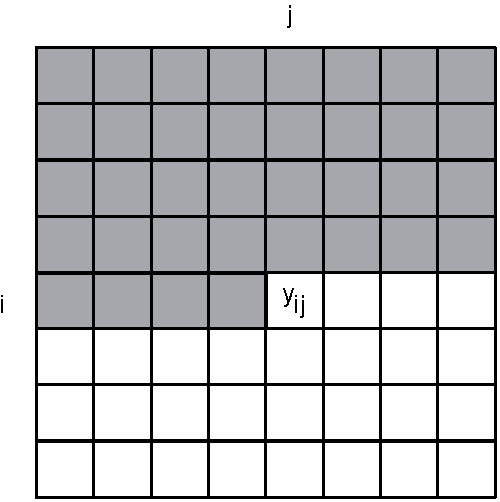
\includegraphics[width=0.3\textwidth]{./figs/conv-a.pdf} &
    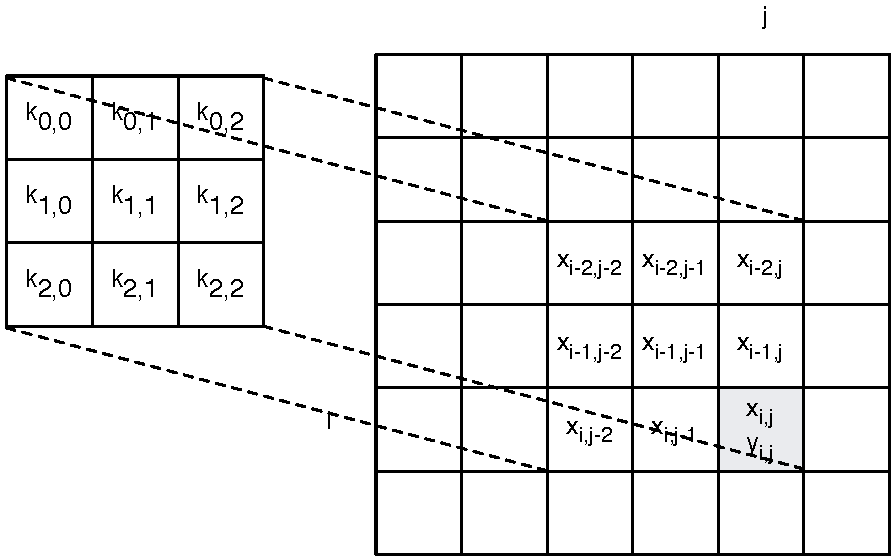
\includegraphics[width=0.5\textwidth]{./figs/conv-b.pdf} \\
-a- & -b-
  \end{tabular}
  \caption{Shifted convolution}
  \label{fig:shifted-conv}
\end{figure}

In certain situations, this ``shifting'' effect is not desirable and one would prefer a more
classical definition of the convolution, in which the convolution kernel is ``centered'' around the
current pixel, as illustrated in Fig.~\ref{fig:centered-conv}. The CAPH standard library therefore
provides ``centered'' versions of 1D and 2D convolutions for several kernel dimensions. The program
\texttt{mkconv}, described in App F of the reference manual, also has an option to generate centered
convolution for any (odd) kernel dimensions.

\begin{figure}[htbp]
\centering
    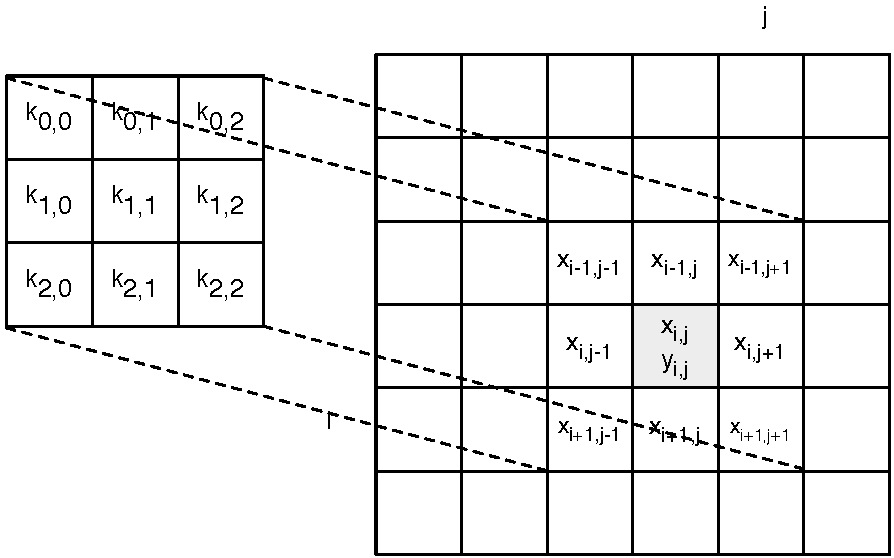
\includegraphics[width=0.5\textwidth]{./figs/cconv.pdf}
  \caption{Centered convolution}
  \label{fig:centered-conv}
\end{figure}

In our case, the only modification is to replace the \verb|conv233| actor in
Listing~\ref{lst:sobel-full} by its centered counterpart \verb|cconv233|. This modification is
denoted in Listing~\ref{lst:sobel-full2} (in which only modified lines have been reproduced).
 
\begin{lstlisting}[style=CaphStyle,numbers=left,caption={Modification of
    listing~\ref{lst:sobel-full} to use \emph{centered} convolution},label={lst:sobel-full2}]
...
net gx = cconv233 ([[1,0,-1], [2,0,-2], [1,0,-1]], 0, 0) i;
net gy = cconv233 ([[1,2,1], [0,0,0], [-1,-2,-1]], 0, 0) i;
...
\end{lstlisting}

\medskip
Simulation results with the interpreter are unchanged, except for the result image, which of course is no longer
shifted and the channel occupation report, as shown in Listing~\ref{lst:sobel-fifo-occ2}.

\begin{lstlisting}[style=BashOutputStyle,caption={FIFO occupation reported by the interpreter for
    the application using centered convolution actors},label={lst:sobel-fifo-occ2}]
W3: occ=0/256 max=107
W2: occ=0/256 max=143
W1: occ=0/256 max=143
W6: occ=0/256 max=107
W5: occ=0/256 max=143
W4: occ=0/256 max=143
W8: occ=0/256 max=2
W7: occ=0/256 max=2
W9: occ=0/256 max=2
W10: occ=0/256 max=2
\end{lstlisting}

Note that, compared with the results obtained with the shifted convolution actors, the occupation of
channels \texttt{W3} and \texttt{W6} can now grow to 107 places. A visualisation of the application
dataflow graph (with the \verb|-dot| and \verb|-dot_show_indexes| options) shows that these channels
are those connecting the \texttt{i} input to the \texttt{cconv233} actors. The reasons for this is
that \emph{centered} convolution actors, contrary to \emph{shifted} convolution actors, requires a
``flushing'' phase at the end of each line of the image and the end of each image. This phase is
needed to empty the FIFOs which are used to memorize previous lines and pixels. During this phase,
no input can be read and if any are available, they accumulates on the FIFOs connected to the actor
inputs. 

\medskip
The same behavior can be observed with the SystemC simulation : the file \verb|main_fifo_stats.dat|
obtained with option \verb|-sc_dump_fifo_stats| reports a maximum occupation of 108 for the two
FIFOs connecting input \texttt{i} to the actors \texttt{cconv233}\footnote{The difference of 1 with
  the value obtained with the interpreter is not significant here.}.  As explained in Sec.~9.5.5 of
the reference manual, this ``accumulation'' effect can be eliminated by inserting \emph{blanking}
clock cycles at the end of each line and each image. If one pixel is injected per clock period, the
amount of horizontal (resp. blanking) for a $M\times N$ convolution should be equal to $N$ (resp
$L\times (M-1)/2$), where $L$ is the width of the input images (number of pixel per column). In our
case, this gives respective values of 5 and 140. This is achieved by modifying the SystemC-related
options in the project file as
illustrated in Listing~\ref{lst:sobel-proj-2}. Note that we also had to increase the ``idle
time'' used to detect the end of the simulation because of the inserted blanking cycles.


\begin{lstlisting}[style=MakeStyle,caption={Modified project file for SystemC simulation (with
    centered convolution actors and blanking)},label={lst:sobel-proj-2}]
...
SC_OPTS = -D ifile=pcb.txt -D threshold=80 -sc_abbrev_dc_ctors -sc_stop_when_idle 2000 -suppress_cast_warnings -sc_dump_fifo_stats -sc_istream_hblank 4 -sc_istream_vblank 140
...
\end{lstlisting}
%$

\medskip
Blanking can also -- and actually should if simulation is expected to reflect ``real'' behavior on the
target hardware, as explained in Sec 9.5.5 of the reference manual -- be simulated at the VHDL
level. For this, the \verb|-vhdl_istream_blanking| must be passed to the CAPH compiler and the
option \texttt{-hblank} (resp. \texttt{vblank}) passed to \texttt{txt2bin} program. This is here
achieved by modifying the project file as illustrated in Listing~\ref{lst:sobel-proj-3}.

\begin{lstlisting}[style=MakeStyle,caption={Modified project file for VHDL simulation (with
    centered convolution actors and blanking)},label={lst:sobel-proj-3}]
...
VHDL_OPTS = -D ifile=pcb.pgm -D threshold=80 -suppress_cast_warnings -vhdl_annot_file main_fifo_stats.dat -vhdl_istream_blanking
...
\end{lstlisting}
%$

%%% Local Variables: 
%%% mode: latex
%%% TeX-master: "caph-primer"
%%% End: 
